\chapter{Evaluación experimental}
\label{cap:evaluacionexperimental}
En el presente capítulo se presenta los resultados obtenidos de las diferentes implementaciones para los métodos propuestos en la secciones anteriores. Se comienza por la implementación de los métodos de procesamiento de transacciones de lectura, posteriormente se muestra los resultados obtenidos para los diferentes métodos de predicción de tiempos de respuestas para consultas y el comportamiento que tienen para diferente conjunto de datos. Finalmente se presenta el comportamiento de las estrategias de planificación presentadas para diferentes tipos de escenarios.

\section{Hardware y conjunto de datos}
\label{evaluacionexperimental:hardwareydatos}
Los experimentos fueron ejecutados en un Intel Xeon E5620 2.4 \textit{Ghz.} con 8 núcleos físicos, tecnología \textit{hyper-threading} y 90 gigabytes de memoria de acceso aleatorio (\textit{RAM}). Se utilizaron dos conjuntos de datos para llevar a cabo los experimentos, estos son frecuentemente usados por la comunidad del área de Information Retrieval. El primero de ellos es \textit{GOV2}, este conjunto es una colección de aproximadamente 25 millones de páginas \textit{Web} obtenida desde los dominios \textit{.gov} y que pesa 426 \textit{GB}. La otra colección de datos utilizada es la \textit{ClueWeb09}, la cual fue creada para apoyar la investigación en recuperación de la información y las tecnologías relacioanadas con el lenguaje humano, consiste en alrededor de un billón de páginas en diez lenguajes diferentes y 50 millones en inglés. \textit{ClueWeb09} pesa alrededor de 5 \textit{TB} en forma comprimidad y 25 \textit{TB} descomprimida. 
% Las consultas (queries)

\section{Wand multithreaded}
\label{evaluacionexperimental:wm}
En esta sección se muestra la implementación de dos enfoques para el procesamiento de consultas a través del algoritmo Wand \citep{Broder:2003}. El primer enfoque es el esquema de \textit{heap} locales (LH), en el que cada hebra obtiene sus mejores documentos para una consulta dada y luego una hebra maestra se encarga de mezclar todos los resultados de cada uno de los hilos de ejecución para construir el conjunto \textit{top-K} final; el segundo enfoque es el enfoque de \textit{heap} compartido (SH), en el que se tiene un \textit{heap} visible a todos los hilos de ejecución y en donde ellos compiten por el acceso a esta estructura de datos. El detalle del diseño de los enfoques LH y SH están disponibles en \ref{scheduling:wlh} y \ref{scheduling:whc}. 

\subsection{Esquema LH}
\label{evaluacionexperimental:esquemalh}
En el esquema LH todos los hilos de ejecución tienen sus propias estructuras de datos y variables que soportan la resolución de una transacción de lectura. La clase \textit{TopKMultithreadWandOperatorLocal} es la encargada de administrar la lógica de ejecución, además prepara las variables e inicia los hilos de ejecución. El Código \ref{code:topkmultithreadwandoperatorlocal} muestra la implementación, en el que existe un método llamado \textit{execute}, este método es el encargado de llevar a cabo la resolución de la consulta, recibe como entrada la consulta a ser resuelta y un vector de resultados, en el que se almacenará los resultados obtenidos. Adicionalmente, este método es el encargado de lanzar las hebras con que se resolverá cada consulta y a cada uno de ellas le asiga un objeto de tipo \textit{TopKWandOperator} ($arr\_ops[pid\_thread]$) para obtener los resultados. Todo este proceso es llevado a cabo usando $K$ como tamaño del conjunto que se quiere obtener. Además se definen variables como \textit{$mapas\_ubs$}, el cual asocia a cada término los \textit{upper bounds} con los que el método Wand trabajará y \textit{$query\_partes$}, variable que define en cuántas partes la consulta debe ser dividia y está supeditada al número de hebras con que esta será resuelta.

\lstinputlisting[label=code:topkmultithreadwandoperatorlocal, caption=Implementación de la clase TopKMultithreadWandOperatorLocal.h, language=C++]{code/TopKMultithreadWandOperatorLocal.h}

En la Figura \ref{fig:esquema_ejecucion_wandsh} se ejemplifica la resolución de una consulta con cuatro hilos de ejecución. Una vez que el sistema asigna el número de hebras que se utilizará para la resolución de la consulta, esta es tomada por el objeto \textit{TopKMultithreadWandOperatorLocal} y hace un llamado al método \textit{execute}, en el que se hace una preparación de variables y se lanzan los hilos de ejecución; cada uno de ellos tiene asignado dos objetos: (1) \textit{TopKWandOperator}, el cual se encarga de que cada hilo de ejecución solo resuelva la parte de la consulta que se le asignó, y (2) \textit{Wand}, el cual se encarga de obtener los mejores $K$ documentos guardándolos en un \textit{heap}.

\begin{figure}[th!]
\centering
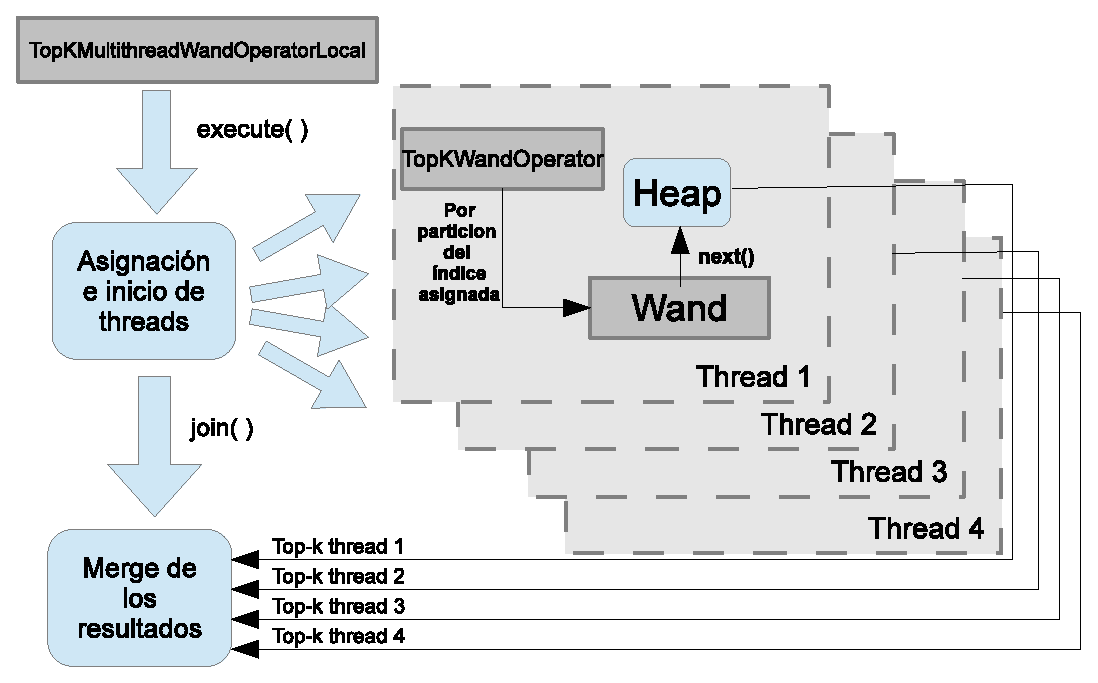
\includegraphics[scale=.75]{images/ejecucion_topkmultithreadwandopLOCAL.eps}
\caption{Esquema de ejecución enfoque LH}
\label{fig:esquema_ejecucion_wandlh}
\end{figure}

\subsection{Esquema SH}
\label{evaluacionexperimental:esquemash}
En el esquema SH los hilos de ejecución trabajan con variables compartidas, incluído el \textit{heap} en donde se almacenan los resultados. La ejecución de este enfoque es llevada a cabo por la clase \textit{TopKMultithreadWandOperatorLocks}, la cual podemos ver en el Código \ref{code:topkmultithreadwandoperatorlocks}; en esta implementación se puede observar la declaración de una clase anidada la que contiene las variables que serán compartidas por los hilos de ejecución. Dentro de las variables más importantes está el \textit{heap}, el umbral utilizado para decidir si un documento debe estar dentro del \textit{heap} y la variable de tipo \textit{mutex} que permite el acceso exclusivo a las variables compartidas. 

\lstinputlisting[label=code:topkmultithreadwandoperatorlocks, caption=Implementación de la clase TopKMultithreadWandOperatorLocks.h, language=C++]{code/TopKMultithreadWandOperatorLocks.h}

La Figura \ref{fig:esquema_ejecucion_wandsh} muestra un ejemplo de resolución de consulta utilizando cuatro hilos de ejecución y el enfoque SH. Al igual que en el esquema anterior, la clase principal inicializa variables e inicia los hilos de ejecución; el objeto \textit{TopKWandOperator} asignará a cada hebra la parte del índice invertido con la que cada hebra resolverá la consulta. Cada vez que un hilo de ejecución utilizando el objeto Wand encuentre un documento candidato para estar en el conjunto \textit{top-K} final, debe pedir acceso exclusivo a las estructuras de datos involucradas (\textit{heap} y umbral), de esta forma se evita resultados erróneos en el conjunto final producto del paralelismo entre los hilos de ejecución.  

\begin{figure}[th!]
\centering
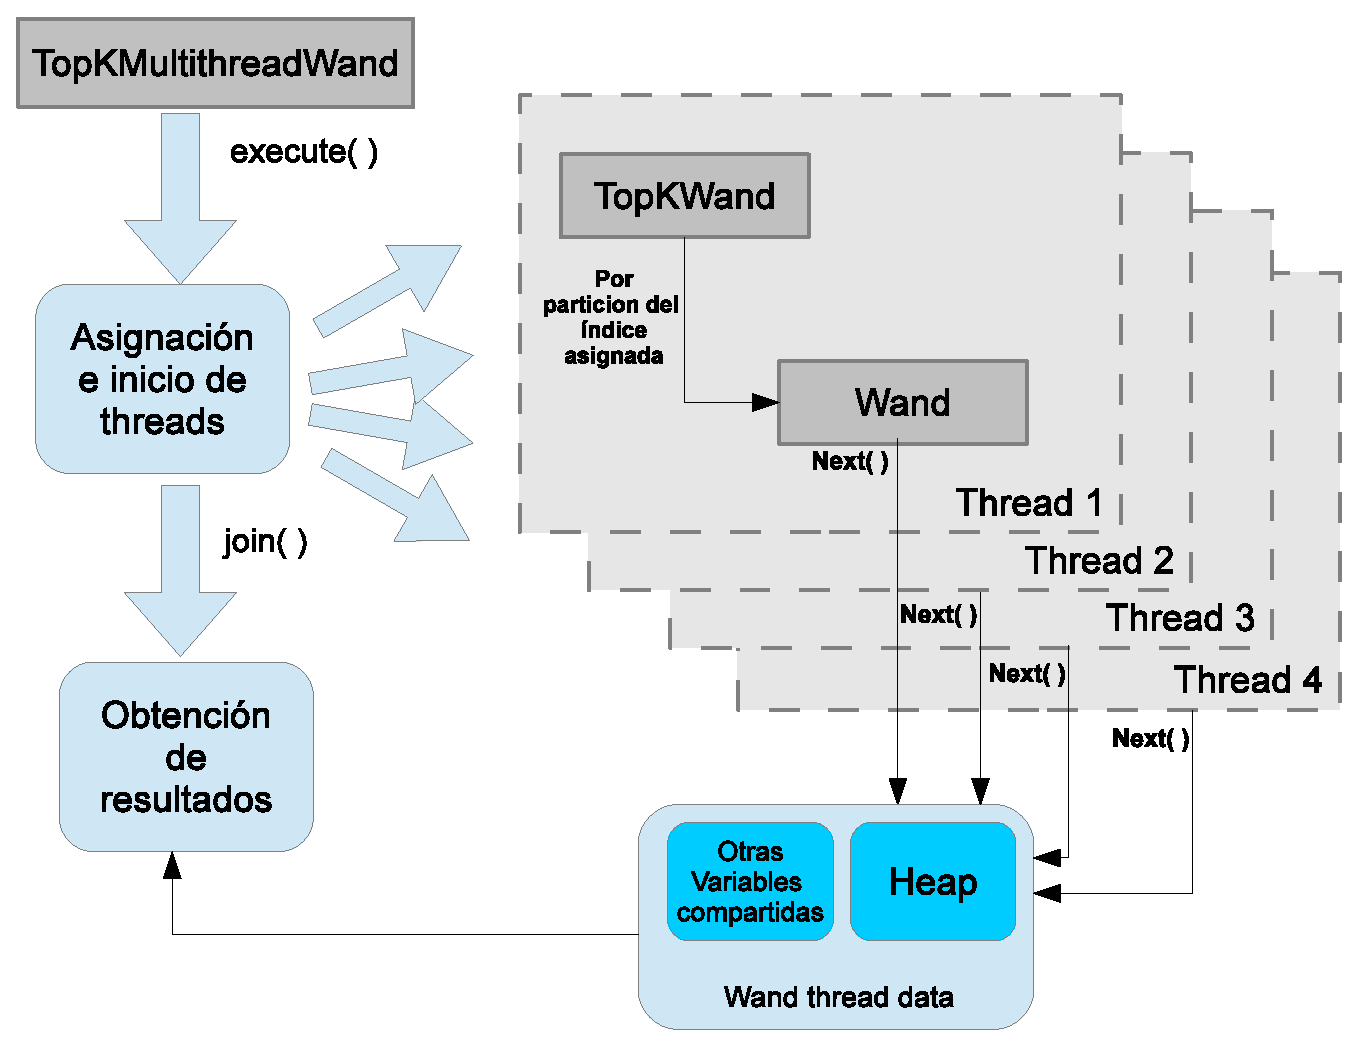
\includegraphics[scale=.75]{images/ejecucion_topkmultithreadwandopCOMPARTIDO.eps}
\caption{Esquema de ejecución enfoque SH}
\label{fig:esquema_ejecucion_wandsh}
\end{figure}


\subsection{Resultados obtenidos}
\label{evaluacionexperimental:resultadosObtenidos}
En la Figura \ref{fig:tiempos_wand} se puede observar el tiempo promedio del enfoque LH y el enfoque SH en resolver un conjunto de 10,000 consultas de la colección \textit{GOV2}. A medida que crece el número de hilos de ejecución, el enfoque de \textit{heaps} compartidos toma ventaja por sobre el enfoque de \textit{heaps} locales, sin embargo, cuando se utiliza un hilo de ejecución se puede observar que LH ($117.486 ms$) requiere un tiempo menor que SH ($130.591 ms$), esto se debe porque en LH no se usa variables compartidas que retrase a los hilos de ejecución esperando a que otros las libere. LH requiere menos tiempo en resolver el \textit{log} de consultas para 2,4,8 y 16 hebras. 
El esquema LH puede estar muy supeditado a la distribución de documentos en las listas del índice invertido, ya que si un hilo de ejecución procesa su corrrespondiente parte del índice invertido en donde los mejores puntajes se encuentran al final, entonces el \textit{heap} tendrá un umbral bajo al comienzo del proceso, eso implica un proceso de descarte de documentos menos eficiente y el tiempo de ejecución requerido será mayor, retrasando el proceso que mezcla los resultados para obtener el conjunto \textit{top-K} final. 
Como el esquema SH ocupa un solo \textit{heap} para obtener los mejores $K$ documentos, el \textit{heap} tiende a llenarse rápidamente con los mejores documentos globales, esto implica que el puntaje mínimo del \textit{heap} (umbral) tiende a crecer rápidamente, permitiendo un mejor descarte de documentos y menor tiempo de ejecución para las hebras. 

\begin{figure}[!ht]
\centering
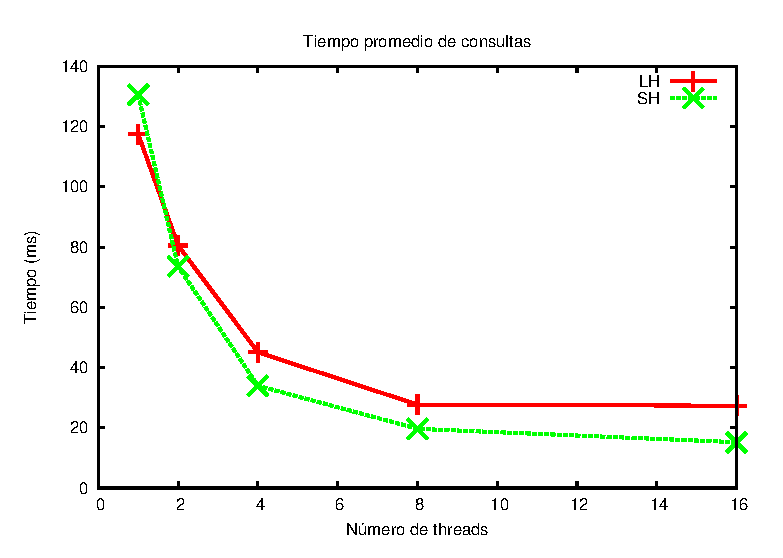
\includegraphics[scale=.75]{images/tiempos_wand.eps}
\caption{Tiempos promedios de las consultas}
\label{fig:tiempos_wand}
\end{figure}

Adicionalmente en la Figura \ref{fig:eficiencias_wand} se puede ver en forma general que con la estrategia de enfoques compartidos se obtiene mejores eficiencias que con la estrategia LH. Con SH la mejor eficiencia que se obtiene es con 4 hilos de ejecución ($0.962 ms$), mientras que con 2 y con 8 hebras se obtiene una eficiencia de $0.887$ y $0.831 milisegundos$; en general se obtiene buenas eficiencias para 1,2,4 y 8 hebras, sin embargo, con 16 hilos de ejecución la eficiencia baja considerablemente ($0.5403$) con respecto a las anteriores, esto se debe principalmente a la tecnología \texti{thyperthreading} de la máquina utilizada. También es interesante ver que el uso exclusivo del \textit{heap} compartido por parte de los \textit{threads} no tiene un fuerte impacto en el rendimiento. La eficiencia baja de LH se debe porque para obtener el conjunto \textit{top-K} final de una consulta debe haber una sincronización de todos los hilos de ejecución involucrados en que cada uno de ellos envíe sus \textit{top-K} locales a la hebra maestra, y además porque existe un costo adicional de calcular el conjunto \textit{top-K} final entre los $P \times K$ documentos seleccionados (siendo $P$ el número de procesadores). 
                     
%Para los siguientes experimentos del presente trabajo se ocupará el enfoque SH para resolver las transacciones de lectura.

\begin{figure}[!ht]
\centering
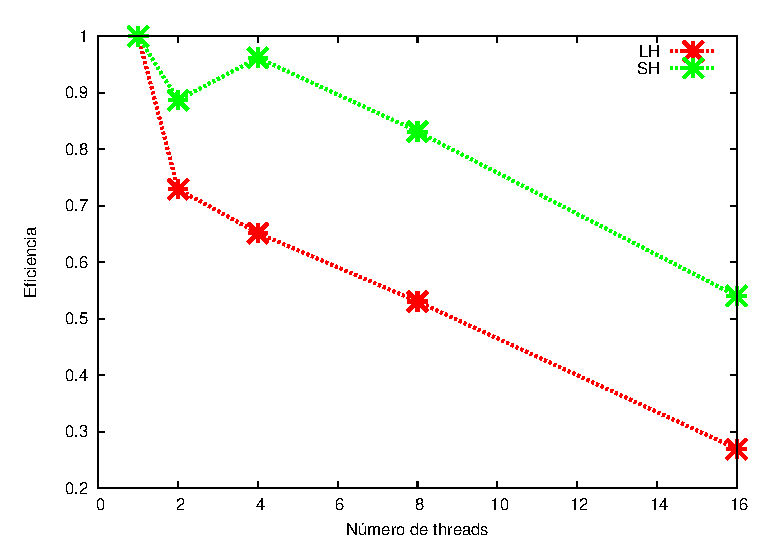
\includegraphics[scale=.75]{images/eficiencias_wand.eps}
\caption{Eficiencias para Wand con heaps compartido y locales}
\label{fig:eficiencias_wand}
\end{figure}

\section{Predicción de tiempos}
\label{evaluacionexperimental:predicciontiempos}
En la Tabla \ref{resultados_glasgow} se puede apreciar los resultados obtenidos con la regresión lineal múltiple con distintos número de hilos de ejecución. Los experimentos se llevaron a cabo utilizando el conjunto de datos GOV2 y el método Wand tradicional. Se llega a buenos valores del coeficiente de determinación a pesar que son 42 variables independientes; todos los valores del coeficientes están sobre el 80%, por lo tanto el modelo representa un porcentaje de variabilidad considerable de la variable independiente, que en este caso es el tiempo en segundos. 

\begin{table}[!ht]
\caption{Resultados obtenidos de la regresión lineal múltiple}
\begin{tabular}{|c|c|c|c|c|c|}
\hline
 & 1 thread & 2 threads & 4 threads & 8 threads & 16 threads \\ \hline
Rcuadrado & 0.7272 & 0,7428135071 & 0,7135704064 & 0,7036605024 & 0,6990570822 \\ \hline
ECM & 7242,4204588977 & 2251,2801134239 & 475,6894968954 & 145,2615752321 & 82,8386825923 \\ \hline
\end{tabular}
\label{resultados_glasgow}
\end{table}


% El estadístico F permite estimar si la relación entre las variables explicatorias y la respuesta es significativa. 
% RMSE



Adicionalmente se implementó un modelo de red neuronal backpropagation, en donde se obtuvieron mejores resultados que en el método basado en la regresión lineal múltiple. 

\begin{figure}[!th]
\centering
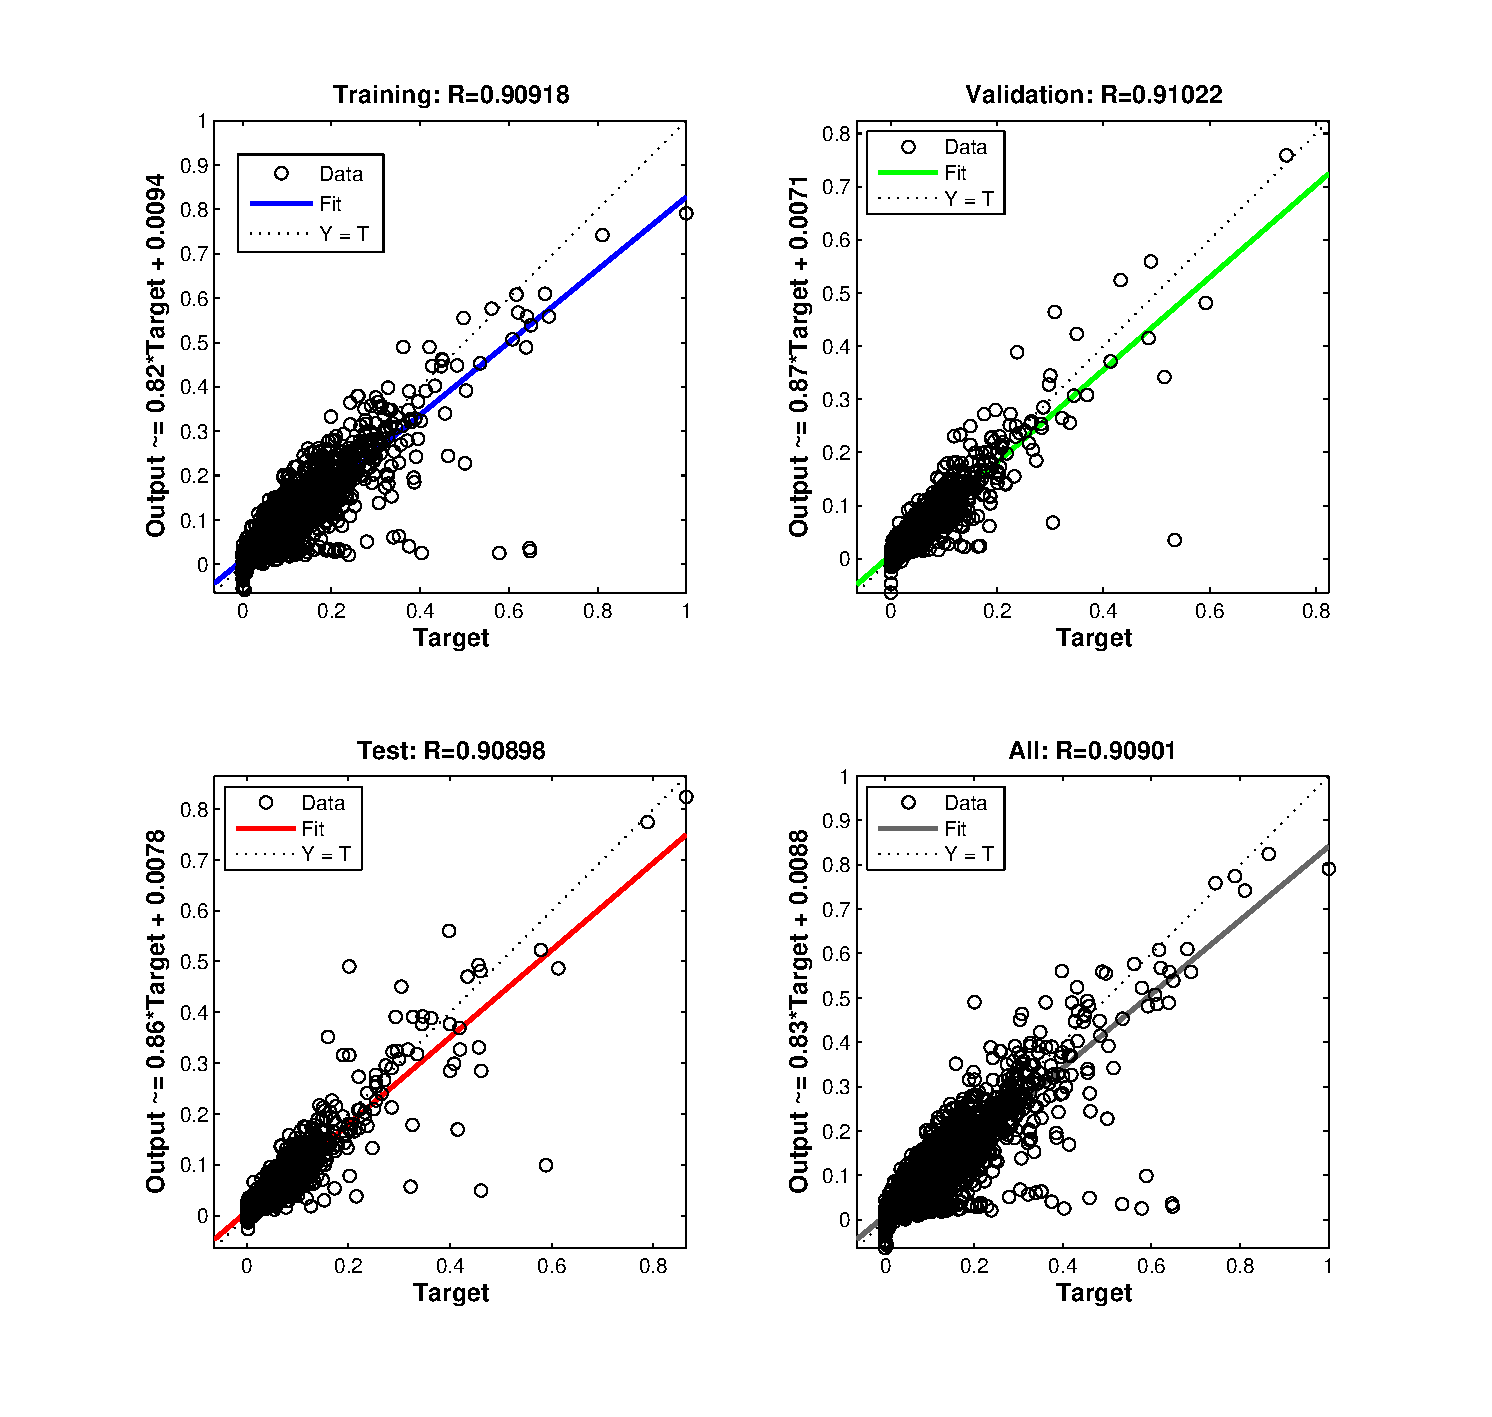
\includegraphics[scale=.75]{images/regresion_backpropagation.eps}
\caption{Regresiones obtenidas por la red neuronal backpropagation}
\label{fig:regresion_backpropagation}
\end{figure}

\begin{table}[htbp]
\caption{Resultados obtenidos de la red neuronal backpropagation}
\begin{tabular}{|l|c|c|c|c|c|}
\hline
\multicolumn{1}{|c|}{} & 1 thread & 2 threads & 4 threads & 8 threads & 16 threads \\ \hline
ECM & \multicolumn{1}{r|}{4593,5493672152} & \multicolumn{1}{r|}{1528,1706707118} & \multicolumn{1}{r|}{335,1918550275} & \multicolumn{1}{r|}{100,0618347161} & \multicolumn{1}{r|}{54,786696642} \\ \hline
\end{tabular}
\label{resultados_redneuronal}
\end{table}








\begin{comment}

// Cómo se llevaron a cabo los experimentos
// Datos
// Máquina
// Programación 


Recordar que en el esquema Wand LH cada uno de los hilos de ejecución computa el conjunto top-K local y luego la hebra maestra hace la mezcla de resultados escogiendo el mejor conjunto top-K global. Este enfoque tiene la ventaja de que es simple de implementar, puesto que no se requiere mecanismos para controlar el paralelismo entre los threads. Sin embargo, se requiere que cada uno de los (P - 1) threads envíe su conjunto solución a la hebra maestra (que también computó su propio conjunto solución), para que crear el resultado final de entre los P x K documentos, donde P es el número de threads encargadas de resolver la consulta y K se es el tamaño del conjunto que se quiere obtener. 

Los resultados en \citep{Rojas:2013} muestran indicios que el esquema LH tendría ventajas por sobre el SH para aquellas transacciones que toman poco tiempo en ser resueltas. 

El Código \ref{code:topkmultithreadwandoperatorlocal} muestra la implementación de la clase que está encargada de llevar a cabo la lógica en la ejecución del enfoque Wand LH. El método execute es el encargado de llegar a cabo la resolución de la consulta, recibe como entrada la query a ser resuelta y un vector de resultados; adicionalmente, este método es el encargado de lanzar los threads con que se resolverá cada consulta y a cada uno de ellos le asiga un objeto de tipo TopKWandOperator (arrops), para obtener los resultados y escribirlos en el vector results. Todo este proceso es llevado a cabo usando el tamaño del conjunto que se quiere obtener (k) y además el índice invertido (indice).


\begin{figure}[!th]
\centering
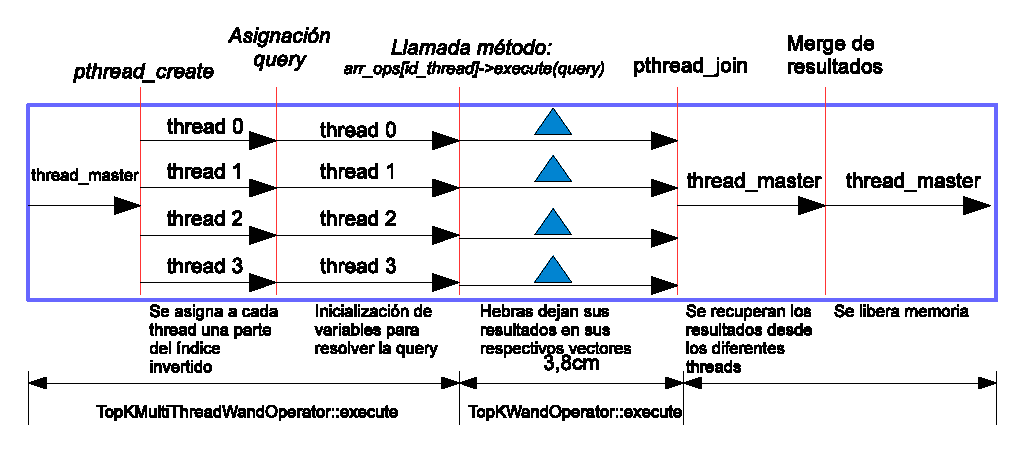
\includegraphics[scale=.75]{images/ejecucion_wandlh.eps}
\caption{Ejemplo de ejecución esquema Wand LH}
\label{fig:ejecucion_wandlh}
\end{figure}

  

%El hecho que en el esquema de heap locales no se requiere mecanismos de control de paralelismo en su implementación, posee ventajas para queries cortas en su procesamiento 
%Figura




\lstinputlisting[label=code:topkmultithreadwandoperatorlocal, caption=Implementación de la clase TopKMultithreadWandOperatorLocal.h, language=C++]{code/TopKMultithreadWandOperatorLocal.h}

Mostrar topK Wand operator

\end{comment}



\begin{comment}

el proceso de descarte tiende a ser más eficiente porque los documentos con mayor puntaje tienden a estar en el heap

Se habla un poco de las ventajas que se tenía con este esquema nuevamente, qué se hizo para la implementación, cómo se programó, etc. 

Se muestra el código y ojalá se muestra algún flujo de ejecución para una query específica.

%\lstinputlisting[language=C++]{code/TopKMultithreadWandOperatorLocal.h}

Se muestra un gráfico y tabla de eficiencia.

\end{comment}




\begin{comment}

Se hace una introducción.

\section{Predicción de tiempo de respuesta a transacción de lectura}
\label{evaluacionexperimental:ptrq}
Se hace experimentos con predictor perfecto

Nosotros optamos por un enfoque de Wand Heap Compartido para ser usado en los experimentos.

Se hace una breve introducción al cpaítulo anterior. 

Se menciona los resultados obtenidos con la regresión, se dice que no se tuvieron muy buenos resultados con la regresión, se deja a ver por qué no se obtuvieron muy buenos resultados (índice con los que se hicieron experimentos, consultas, etc.).

\begin{table}[H]
\centering
\caption{Resumen de los estadísticos que se deben extraer desde el índice invertido}
\label{tabla:estadisticosGlasgow}
\begin{tabular}{|l|}
	\hline
	\textbf{Estadísticos del término s(t)} \\	
	1. Media aritmética	 \\ \hline
	2. Media geométrica	 \\ \hline
	3. Media harmónica	 \\ \hline
	4. Puntaje máximo	 \\ \hline
	5. Varianza del puntaje	 \\ \hline
	6. Número de documentos	 \\ \hline
	7. Número de máximos	 \\ \hline
	8. Número docs > media	 \\ \hline
	9. Número docs = máximo puntaje	 \\ \hline
	10. Número docs dentro del 5\% más alto	 \\ \hline
	11. Número docs dentro del 5\% del umbral	 \\ \hline
	12. Número de inserciones al conjunto top-K	 \\ \hline
	13. IDF	 \\ \hline
	14. Tiempo en resolver $t$ como \textit{query}	\\ \hline  
\end{tabular}
\end{table}


	//menos que 10% tpo esperado, menos que 25%, menos que 50% y el resto (en el timesRanges)
\subsection{Predictor perfecto}
\label{evaluacionexperimental:predictorperfecto}

Decir que no es el foco de esta tesi, que los resultados obtenidos no fueron muy buenos s y que para evaluar los algoritmos de scheduling  también se usará un predictor perfecto. Decir cómo se obtuvo un predictor perfecto y ojalá mostrar algún algoritmo.





\section{Estrategias de scheduling}
\label{evaluacionexperimental:estrategiasscheduling}

Hablar separado cada una de ellas, mostrando implementación y cómo se llevaron a cabo los experimentos.

1. Comparar las tres estrategias de scheduling (decir que TimesRanges es mejor) ==> Con predictor perfecto también?
2. Comparar TimesRanges con baseline ==> Con Predictor perfecto también.  
4. Decir los problemas que existen en cada una de las estrategias que se pierden tiempos.
3. Sacar a la luz la nueva unidades de trabajo ==> Predictor perfecto también.
4. Comparación unidades de trabajo - baseline - TimesRanges.

Conclusiones para cada uno de los gráficos realizados. 

Se intuye que habrá pérdida de eficiencia al final de cada bloque en FR.

\end{comment}